\documentclass[preprint,12pt]{elsarticle}
\usepackage{graphicx}
\usepackage{amssymb}

\journal{CS4701 - Bart Selman}

\begin{document}

\begin{frontmatter}
	\title{3D Tic-Tac-Toe}
	\author{Lillian Chen (qc53) \& Jim Yu (jly29)}
	\address{Cornell University}

	\begin{abstract}
		In the interest of exploring the application of game tree problems, we have implemented a 3-dimensional tic-tac-toe game and an artificially intelligent player in python. This paper will include a clear description of the overall goals of the project, the software written, and the results of an evaluation of our system with various observations on the AI components and their performance.
	\end{abstract}
\end{frontmatter}

\section{Introduction}
	The goal of our project is to understand game trees through a deterministic, turn-taking, two-player, zero-sum game of perfect information. In order to do this, we created an AI player for a 3D tic-tac-toe game that optmizes its total number of wins over time. This AI will not be given any prior strategies and instead must rely on its game tree, where each node represents a board position and the children of each node are the legal moves from that position. The more games our computer plays, the more complete the tree will become and therefore the better a player the AI will be.

	As we implement this AI, we will keep in mind additional goals in best utilizing the space and runtime available on an average computer. Due to the academic purposes of this project, we expect the game to be able to run on our laptop for all possible demonstrational and educational usages. This will also help us develop further as software engineers to be able to ship working code while keeping in mind the impact of efficiency.

\section{Game Analysis}
	3D tic-tac-toe is a two player game that slightly modifies the rules of the original tic-tac-toe game by presenting a different board setup. Rather than one 3x3 board where players X and O can each place their moves, 3D Tic-tac-toe essentially has three 3x3 boards on top of each other such that the method to win now changes. (Note, however, that the center tile of the middle board is an invalid space. More on this in Section 2.2.) The goal of the game then is still to reach three respective marks in a row but now this row can line up vertically, horizontally, or diagonally on either a single board or across all three.

	\subsection{Play Mechanics}
		Upon initiation, the game begins at the menu, where there are three buttons: play, learn, and about (figure 1). The about option is a simple text screen giving brief credits and information about the project.

		\begin{figure}[h]
			\centering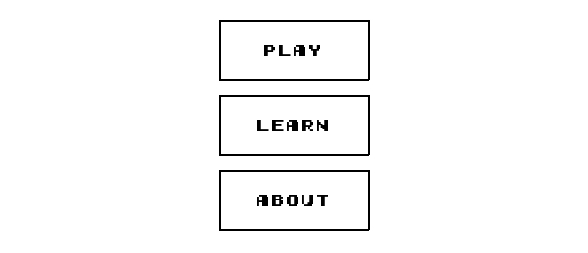
\includegraphics[width=0.5\linewidth]{0.jpg}
			\caption{main menu}
		\end{figure}

		The play option (figure 2) is the human versus computer mode, the former represented by an X and the latter an O. The human player is given a prompt prior to starting the game to choose whether he would like to make the first move. The game then begins and displays three 3x3 boards representing the top, middle, and bottom board in that order. Depending on the player's earlier choice, an O, representing the computer's move, will be on the board. At this point, the human player is free to use the mouse and click on a tile for his own move. All inputs outside of a tile, on the center tile of the middle board, or on a tile already chosen by either player are invalid and will not be registered. This repeats until some player achieves 3 consecutive marks in a row and wins, after which the human player is directed back to the menu.

		\begin{figure}[h]
			\centering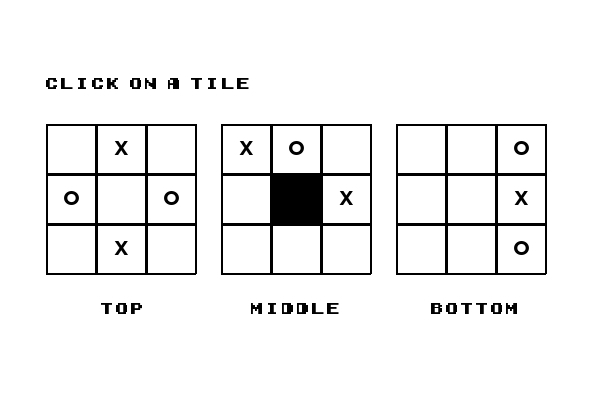
\includegraphics[width=0.5\linewidth]{1.jpg}
			\caption{play mode displaying top, middle, bottom boards}
		\end{figure}

		The learn option is essentially the same as the play mode but the computer plays against itself in order to fill its game tree data further. Games between the computer players will repeat until prompted to stop, therefore allowing the program to be left alone for an extended period of time to reach an optimal AI player. The proceedings of these games, however, will not be visually available on the GUI due to the high speed that the computers will be playing each other. Instead, it will be running in the background.

	\subsection{Omission of Center Tile}
		The choice to leave out the center tile on the middle board was made in order to avoid an extreme advantage given to the player who chooses to take the space.

		If the center tile was not omitted, there would be 49 distinct 3-in-a-rows, given that there are 8 on each board, 9 vertically stacked columns, and 16 diagonally configured rows stretching across all three boards. Of these, there are 12 rows that include the center tile, making them approximately a quarter of the winning rows. Therefore, if the first player takes this space, he will be eliminating a quarter of the possible positions to win for his opponent.

		However, the higher worry is that an intelligent human player can take advantage of the board to force a win for himself regardless of the actions of the opponent. The strategy for this win can span as little as 7 total actions because given the prompt to make the first move, the human can respond yes and immediately occupy the center tile. Then, whichever tile the AI chooses, the human can respond with a move that forces the AI to counter it in its next turn. Very soon, there will reach a point where there are more than one spaces for the human player to win and the AI not being able to block all of them in one turn will be ensured a loss (figure 3). With this strategy in place then, the computer will have no chance with or without artificial intelligence, rendering the purpose of this project moot.

		\begin{figure}[h]
			\centering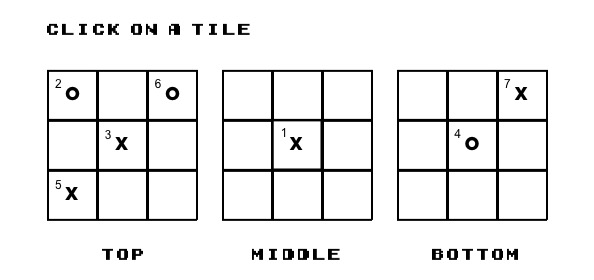
\includegraphics[width=0.75\linewidth]{3.jpg}
			\caption{winning strategy with a center tile, each mark is numbered in order of play}
		\end{figure}

		Of course, if the human player is unaware of this winning strategy, the computer can also take advantage of it without meaning to do so. This is because as the AI fills its game tree, it can easily find the routes corresponding to this strategy as the terminal state is reached at 7 moves. And with the guaranteed victory of these series of steps, the AI as we implemented it will always take the move leading to the outcome with the highest history of wins, therefore influencing the computer over time to utilize this strategy without ever having known about it.

		For this reason, we have omitted the center tile in order to test the full ability of our AI player without taking advantage of the board itself. We believe this will allow us to explore the depths of our subject further and fulfill our intended goal in a more meaningful way.

	\subsection{Impossibility of Ties}
		An interesting variance from the original 3x3 tic-tac-toe is that there are no ties in this version. The outcome of a tie is incredibly common for the oriignal game if both players are able to counter each other appropriately and fill up all 9 tiles of the small board. However, a tie in 3D tic-tac-toe is actually impossible, although we will not go deeply into the proof of why in ths paper because it is less relevant to our project. However, to summarize, in order for a tie to exist, each three of the boards must contain a tie within itself. Then when lining these boards up, there will always exist some winning row due to the nature of the game and the symmetry of Xs against Os (figure 4).

		\begin{figure}[h]
			\centering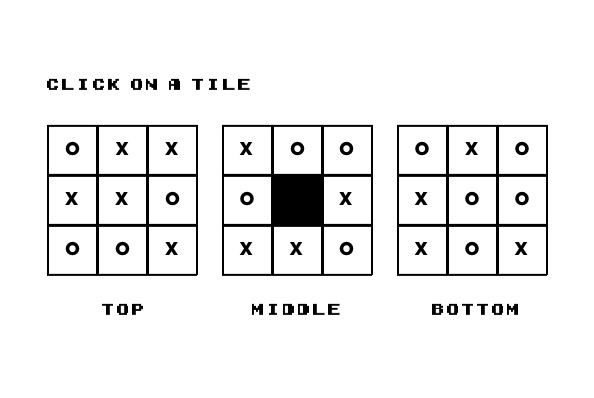
\includegraphics[width=0.5\linewidth]{2.jpg}
			\caption{despite a tie on each board, there are multiple winning rows in the configuration above}
		\end{figure}

		The result of this fact then is meaningful to us in that every game will alter the game tree in some way because it will always be a win or a loss. Having a definite winner then changes the weights of the moves corresponding to each game, either causing the AI player to veer away from them as they are now less likely to lead to a win or incline towards them as they've been proven to gather more wins. This therefore makes our implementation not only less complex but also more effective.

\section{Code Structure}
	The game itself is developed with python using pygame, a set of modules specifically meant for game development. A breakdown of our code structure is as follows:

	\begin{itemize}
		\item main.py: mainly handling the GUI, includes the menu, gameplay, and about page
		\item board.py: backend configuration of gameplay, updating the board per legitimate move and checking whether a winner exists
		\item bot.py: the AI player which searches its game tree for the best next move and fills it in learning mode
	\end{itemize}

	The overall game is broken in 6 states: \textbf{begin}, \textbf{choose}, \textbf{play}, \textbf{learn}, \textbf{about}, \textbf{end}, \textbf{learn\_end}. While the game is running, main.py switches between appropriate states as follows:

	\begin{itemize}
		\item \textbf{begin}: main menu
		\item \textbf{choose}: after clicking play in \textbf{begin}, prompts the user on whether he wishes to make the first move
		\item \textbf{play}: human versus AI gameplay
		\item \textbf{learn}: iterates through AI versus AI games in the background in order to fill in tree
		\item \textbf{about}: credits
		\item \textbf{end}: displays results when a winner is declared at the end of the \textbf{play}
		\item \textbf{learn\_end}: prompts the AI to add the results of \textbf{learn} into its game tree and initializes a new game
	\end{itemize}

\section{AI Approach}
	In this section, we will most consider the goals that we've declared: optimizing the AI's overall wins with a game tree, the time to process each next move, and the space consumed in our memory.

	\subsection{Minimax Implementation}
		Given the game is two-player, we would normally utilize a minimax algorithm but because the human player has the choice of who goes first, we cannot assign MAX and MIN as easily to either player.

		\begin{figure}[h]
			\centering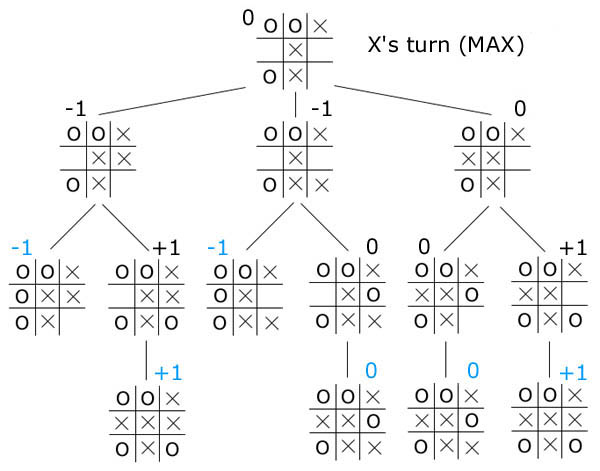
\includegraphics[width=0.75\linewidth]{4.jpg}
			\caption{portion of game tree for a normal 3x3 tic-tac-toe game, where -1 is a loss, +1 and a win, and 0 is a tie for MAX. Next to each node is its heuristic by a normal minimax algorithm.}
		\end{figure}

		Instead, for the purposes of our project, the AI player will always be MAX, whether or not it takes the first move. Rather than alternating down the game tree then, we must simply find the current state in the tree and always take the maximum heuristic. This method is very similar to the breadth-first search.

	\subsection{Looking Ahead}
		In order to determine a next best move, our AI player will look at all the immediate children nodes from the current board state. Then it will iterate through a number of steps.

		First, the AI will determine whether some terminal state exists among the children nodes. If at least one does, it will check there exists a terminal state in favor of the AI. If so, it will make the winning move. If there only exist lossing terminal states, then it will take the opponent's winning move. The best case scenario is that there was only one terminal state and that prevents the opponent from winning. Otherwise, if the opponent has more than one winning move, then the AI will lose no matter what. However, since encountering this situation is a guaranteed loss for the AI, it should cause the nodes leading to the corresponding terminal state to have a lower heuristic as it learns from past losses. (The calculation of the heuristic will be explained in the next section.) Therefore, while there is nothing we can do once it reaches this point, it will still be a positive influence for future games.

		Next, if there do not exist any terminal states among the immediate children nodes, then the AI will choose the move with the highest heuristic. Ties are broken via random selection (so essentially, prior to first entering learning mode, the AI is simply randomly selecting an available tile each time it makes a move). Ideally, this will lead the AI to a terminal state where it has won many times in the past.

		As an afterthought to Section 2.2, we could have solved the issue with a 4x4x4. However, after considering the factors in this section, we decided to simply omit the center tile instead because the number of children nodes for each state only grows exponentially as the possible moves are heavily increased. With a 3x3x3, there are 26 total tiles for either player to claim. However, a 4x4x4 would have 64 available spaces, almost 2.5 times more than that of 3x3x3. This would therefore only put an incredible amount of stress on our runtime and space when we can simply omit the center tile.

		Another consideration that comes to mind is how far the AI should look into the future. Of course, the farther it looks, the better the next move will be as it can predict a better future. However, even at the 3x3x3 configuration we have now, we must restrict ourselves to one step ahead if we wish to keep the search and insert runtime fast and the space small. This is because we must look ahead an odd number of steps so that it corresponds to when it is the computer's turn to make a move again. Therefore, we would not only increase the number of states to consider exponentially but also in multiples of 2. This, we decided, was not worth the loss of space and the drag in runtime because we are aiming for optimal \textit{overall} wins. So although we may run into a trap of inevitable loss where the opponent will have more than one winning move, we will count on the heuristics to avoid them more and more as the AI learns over a long period of time.

	\subsection{Heuristic}
		The heuristic that we use is a little different than its default definition and features, as we do not recalculate the heuristic for each considered move immediately after an action. Instead, it is stored in the tree and adjusted upon termination of each game. It is a little similar, however, in that it is dependent on some terminal state for its calculation and that it helps immensely in deciding the next best move to take.

		The heuristic for each board state changes according to its involvement in a win or loss. Upon initiation, all heuristics in the game tree are equal to 0. At the end of each game in learning mode, however, the heuristic for all the moves leading to the terminal state is defined as follows:

		\begin{equation}
			heuristic[state] += ((1.0/n) + 1) * outcome
		\end{equation}

		Let $n$ be the number of nodes to the terminal state and the $outcome$ be -1 if the AI loses and +1 if it wins. In this respect, the node's heuristic increases or decreases corresponding to how close it was to the terminal state, with the closest being the largest impact. Note that all moves unassociated with the terminal state should remain the same.

\section{Further Work}
	Although we were given a full semester to work on this project, we admit that there are definitely still ways to improve.

	\subsection{Alpha-Beta Pruning}
		The problem with our algorithm is that the number of game states it has to examine is exponential to the breadth of our tree. If we had used the original minimax algorithm, where game states increase exponentially to the depth of the tree instead, alpha-beta pruning would have been more straightforward in cutting down the number of states. Unfortunately, because of the way we've implemented our search algorithm, this would not apply and we still have to look through the entire breadth for the best heuristic stored.

		However, if we were able to find a depth dependent algorithm instead (it does not necessarily have to exactly be minimax), we would easily be able to use pruning and gain greater freedom to many of the restrictions we set ourselves here. This would have been particularly beneficial asset to enable the AI to look further ahead in the game tree for even more optimized moves. Unfortunately, we were not able to do so in time and therefore could not take advantage of any type of pruning.

	\subsection{Space Reduction with Recursion}
		Similarly to the alpha-beta pruning, we found that had we used a depth-dependent strategy, we could have greatly reduced memory consumption using recursion to represent the tree. However, our hashtable is still quite efficient so this was not too large of an issue.

	\subsection{Game Tree GUI Representation}
		The largest reason for this project was to improve our understanding of the game tree, which we certainly have obtained a firmer grasp of by implementing 3D tic-tac-toe. However, it would have been both very interesting and educational to have represented the tree in the GUI during learning mode. We chose not to display the actual proceedings of the game while the computer were playing against itself because of how fast it is done but at the same time, we are left with very little feedback as to how well our AI player is actually learning. We are only able to subjectively evaluate the AI's improvement by playing it before and after some learning session. However, seeing the AI fill the tree would have definitely shown the caliber of our work in a clearer way.

\section{Evaluation}
	To evaluate the success of our algorithm, we tested our AI against both itself and human players (such as ourselves). In this evaluation process, we ran different strategies to determine the most optimal one, such as a different method to break a tie in heuristics.

	Through observations and winrates, we saw that the AI made reasonable moves to bring it closer to victory. We also found the AI to be efficient as we stored the game tree in a hashtable, which has a time complexity on average of O(1) and worse cast of O(n). We also observed that the best path to victory entails that the AI does not make unnecessary moves when there is a shorter path to a win state.

	Lastly, we reflect on our decision to use python for our implementation and decided that, particularly with the help of Pygame, making the game itself was very easy. As a pencil and paper game, tic-tac-toe was a perfect way to utilize Pygame's simplistic modules. The only worry is that we did mention that part of our goal was the universality of our game to be used on any average computer and Pygame, unfortunately, is highly incompatible with updated operating systems. It also comes with an enormous amount of dependencies for the installation and so takes a heavy toll on the host computer. So while we may have optimized the space and runtime of the game itself to the best of our ability, we may have jeopardized satisfaction of the goal using the very tools we used to build it.

\section{Conclusion}
	With the 3D tic-tac-toe application as described in this paper, we feel that we have satisfied the goals we've set for ourselves at the beginning of this project. Although a very simple game, it made for a great method for us to thoroughly explore the means of executing a game tree with efficiency and performance in mind.

\end{document}